\documentclass[10pt]{article}

\usepackage[letterpaper,margin=0.5in]{geometry}
\usepackage{amsmath,amssymb}
\usepackage{graphicx}
\usepackage{hyperref}
\usepackage{microtype}
\setlength{\parindent}{0pt}
\setlength{\parskip}{4pt}
\linespread{0.94}
\usepackage[font=footnotesize,labelfont=bf,skip=3pt]{caption}
\usepackage{tikz}
\usepackage{pgfplots}
\pgfplotsset{compat=1.18}
\usetikzlibrary{arrows.meta}

\hypersetup{colorlinks=true, linkcolor=blue, citecolor=blue, urlcolor=blue}
\setlength{\emergencystretch}{3em}
\allowdisplaybreaks

\definecolor{figblue}{HTML}{2A6FB0}
\definecolor{figorange}{HTML}{D1622B}
\definecolor{figteal}{HTML}{1D9E75}
\definecolor{figpurple}{HTML}{534AB7}
\definecolor{figink}{HTML}{242424}
\definecolor{figboxgray}{HTML}{A0A0A0}
\definecolor{figlightgray}{HTML}{E8E8E8}
\definecolor{figpaleteal}{HTML}{E8F4F0}
\definecolor{figpalepurple}{HTML}{F1EEFB}

\pgfplotsset{
  every axis/.append style={
    line width=0.5pt,
    axis line style={black!70},
    tick style={line width=0.4pt, black!60},
    label style={font=\small},
    tick label style={font=\footnotesize},
    legend style={font=\footnotesize, draw=none, fill=none},
  },
}


\setlength{\abovedisplayskip}{5pt}
\setlength{\belowdisplayskip}{5pt}
\setlength{\emergencystretch}{1.5em}
\newcommand{\head}[1]{\par\vspace{5pt}{\fontsize{11}{12}\selectfont\bfseries #1}\par\vspace{2pt}}
\captionsetup{hypcap=false}
\newcommand{\figcap}[1]{\captionof{figure}{#1}}
\hypersetup{pdftitle={Solving Drop the Handkerchief},pdfauthor={James Cenawood}}
\begin{document}
{\LARGE\bfseries Solving Drop the Handkerchief}\par
James Cenawood \hfill September 11, 2026
\vspace{4pt}

With optimal play, the first Dropper wins about \textbf{54.49\%} of games under the survival rule below.
We compute the values of all \textbf{289 million state classes} in a backward pass.

\begin{minipage}[t]{0.55\textwidth}
\vspace{0pt}
\head{1. The game}
In the final arc of Toshio Sako's \emph{Usogui}, Surpassing the Leader, two players take part in a deadly game: Drop the Handkerchief.
One player sits in a chair, while the other stands behind them holding a handkerchief.
A minute timer begins, and the player holding the handkerchief must drop it, and the seated player must check if it is on the ground.
If a player checks and the handkerchief is on the ground, the difference is injected into their cylinder. If it is not, their full accumulated cylinder + an additional
60 seconds is injected as penalty. Whoever dies first loses. That is the full game.
For each player, $s$ is squandered time (ST), the seconds in their cylinder; $t$ is total time dead (TTD), the sum of prior doses.
We represent the state as $x=(s_c,t_c,s_d,t_d)$, with Checker first.
Both start at $(s,t)=(0,0)$.

If the Dropper chooses $d\le c$, the Checker succeeds and adds
$\ell=c-d+1$ to ST. At $s_c+\ell\ge300$, the Checker loses.
Otherwise, they swap roles:
$x_\ell=(s_d,t_d,s_c+\ell,t_c)$.
If $d>c$, the Checker receives an injection of $s_c+60$ seconds.
They survive with probability
\[
p(s,t)=\begin{cases}
0.95(1-s/240)\,0.75^{t/60},&s\le239,\ s+t\le240,\\
0,&\text{otherwise}.
\end{cases}
\]
On revival, ST resets, TTD gains the dose, and the players swap roles:
$x_f=(s_d,t_d,0,t_c+s_c+60)$. Otherwise, the Checker loses.
We choose this probability formula for the model; the manga does not specify it.

\head{2. Equivalence Class}
We denote a profile \emph{failure-fatal} if its next failed check means death ($p=0$).
We keep its ST and replace its TTD with a sentinel marker $\bot$.
This grouping is the \emph{quotient}:
\[
\varphi(s,t)=\begin{cases}(s,t),&p(s,t)>0,\\(s,\bot),&p(s,t)=0.\end{cases}
\]
\textbf{Proof.} A successful check raises ST, so a failure-fatal player
remains failure-fatal. Their exact TTD affects neither the loss on failure
nor the grouped state after success. For each action pair, two states in
the same group therefore have the same loss probability and next group.
Backward induction gives them the same value. \textup{QED}

From the start, TTD stays in $\{0,60,61,\ldots,300\}$:
a revival adds at least 60 and cannot exceed 300.
Of $300\times242=72{,}600$ profiles, we keep
$240+\sum_{t=60}^{240}(241-t)=16{,}711$ with $p>0$, plus 300 markers.
For two players, we reduce $72{,}600^2$ states to
$17{,}011^2=289{,}374{,}121$ classes.

\head{3. Backwards Sweep}
We order the classes by a progress score,
\[
\Phi=s_c+s_d+\rho_c+\rho_d,\qquad
\rho(s,t)=\begin{cases}t,&p>0,\\301,&p=0.\end{cases}
\]
\textbf{Proof of termination.} Success adds $\ell\ge1$ to
$\Phi$, or $\ell+301-t>0$ on becoming failure-fatal.
After revival, the increase is 60 if survival remains possible,
or $301-(s+t)\ge61$ otherwise. Role swaps preserve the score.
Since $0\le\Phi\le1200$, play ends within 1,201 steps.
We solve from layer 1200 down to 0, using known later values. \textup{QED}

\end{minipage}\hfill
\begin{minipage}[t]{0.42\textwidth}
\vspace{0pt}
\centering
\includegraphics[width=\linewidth,trim=100 10 95 0,clip]{build/figures/seaborn/fig1_revival_probability.pdf}
\figcap{Revival becomes less likely as either time total grows. Beyond $s+t=240$, the player cannot survive; at $s=240$, revival also has probability zero.}
\vspace{10pt}
\includegraphics[width=\linewidth]{build/figures/seaborn/fig2_toeplitz_structure.pdf}
\figcap{Each diagonal has one success payoff $S_\ell$; each failed check has payoff $F$. We need at most 61 values for the 3,600 action pairs.}
\vspace{12pt}
\resizebox{\linewidth}{!}{
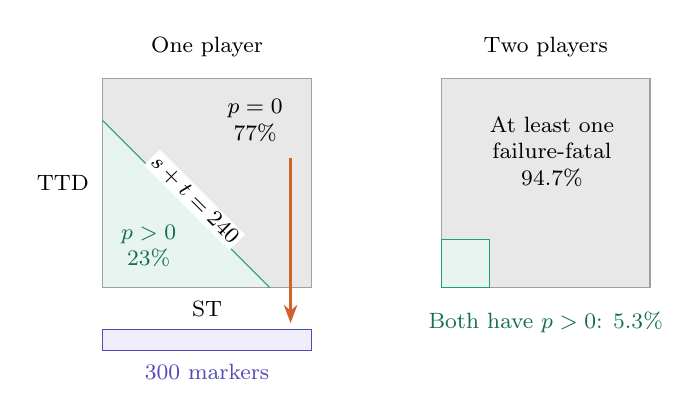
\begin{tikzpicture}[x=0.53cm,y=0.53cm,every node/.style={font=\footnotesize}]
\fill[figlightgray] (0,0) rectangle (5,5);
\fill[figpaleteal] (0,0)--(4,0)--(0,4)--cycle;
\draw[figboxgray] (0,0) rectangle (5,5);
\draw[figteal] (4,0)--(0,4);
\node[rotate=-45,fill=white,inner sep=1pt] at (2.2,2.1) {$s+t=240$};
\node[text=figteal!70!black,align=center] at (1.1,1.0) {$p>0$\\$23\%$};
\node[align=center] at (3.65,4.0) {$p=0$\\$77\%$};
\node[anchor=east] at (-0.1,2.5) {TTD};
\node[anchor=north] at (2.5,-0.1) {ST};
\filldraw[fill=figpalepurple,draw=figpurple] (0,-1.5) rectangle (5,-1);
\draw[-{Stealth},figorange,thick] (4.5,3.1)--(4.5,-0.85);
\node[anchor=north,text=figpurple] at (2.5,-1.6) {300 markers};
\node[anchor=south] at (2.5,5.3) {One player};
\begin{scope}[xshift=4.3cm]
\filldraw[fill=figlightgray,draw=figboxgray] (0,0) rectangle (5,5);
\filldraw[fill=figpaleteal,draw=figteal] (0,0) rectangle (1.15,1.15);
\node[align=center] at (2.65,3.25) {At least one\\failure-fatal\\$94.7\%$};
\node[anchor=north,align=center,text=figteal!70!black] at (2.5,-0.35) {Both have $p>0$: $5.3\%$};
\node[anchor=south] at (2.5,5.3) {Two players};
\end{scope}
\end{tikzpicture}
}
\figcap{We merge the grey profiles with the same ST. Both players remain alive. The left panel sketches the region.}
\end{minipage}
\newpage
\begin{minipage}[t]{0.55\textwidth}
\vspace{0pt}
\head{4. Computing both players' strategies}
Let $V$ be the current Dropper's win probability minus loss probability.
The win probability is $(1+V)/2$. A role swap negates $V$. With the next states from Section 1, set
\[
S_\ell=\begin{cases}1,&s_c+\ell\ge300,\\-V(x_\ell),&\text{otherwise},\end{cases}
\]
\[
F=\begin{cases}1,&p=0,\\1-p-pV(x_f),&p>0.\end{cases}
\]
For drop second $d$ and check second $c$, the payoff is
\[
M_{d,c}=\begin{cases}S_{c-d+1},&c\ge d,\\F,&c<d.\end{cases}
\]
The players can randomize their seconds. Their probability vectors
$a,b$ give $V=\max_a\min_b a^{\mathsf T}Mb$.
The finite matrix minimax theorem guarantees this value.
We first test a single-second support: if the best row minimum equals the smallest column maximum, those choices solve the round outright in O(60).

For a full support, we find a pair that makes the opponent indifferent between seconds,
put $D=S_1-F$ and $\Delta_m=S_{m+1}-S_m$. For $D\ne0$, compute
\[
\boxed{r_1=1,\qquad r_k=-\frac{1}{D}\sum_{m=1}^{k-1}\Delta_m r_{k-m}
\quad(2\le k\le60).}
\]
If the weights are finite and nonnegative, normalize them:
$a_k=r_k/\sum_j r_j$ and $b_k=a_{61-k}$.

\textbf{Proof of the recurrence.} Subtract adjacent rows:
\[
(Mb)_d-(Mb)_{d+1}=D b_d+\sum_{m=1}^{60-d}\Delta_m b_{d+m}.
\]
Set this to zero and start from $b_{60}\propto1$ to obtain the recurrence.
Column differences give the same weights in reverse order.
Thus both players equalize the opponent's payoffs and form an equilibrium.
If we clip negative weights to zero, we must check the new pair. \textup{QED}

\head{5. Error Bounds}
For any probability vectors $a,b$, set
$L=\min_c(a^{\mathsf T}M)_c$ and $U=\max_d(Mb)_d$.
The Dropper guarantees $L$; the Checker limits the payoff to $U$.
Thus $L\le V\le U$ for this matrix.
We require $U-L\le10^{-6}$ and store the midpoint, or a center
with a proved error of at most $5\times10^{-7}$.

\textbf{Proof of the total bound.} A child-value error of at most $e$
changes an expected payoff and the matrix value by at most $e$.
Each step adds at most $5\times10^{-7}$.
Induction over the layers gives
$|\widehat V-V|\le(1201-\Phi)5\times10^{-7}$. \textup{QED}
These are numerical bounds for the stated model; the full-matrix
fallback uses floating-point checks.
\end{minipage}\hfill
\begin{minipage}[t]{0.42\textwidth}
\vspace{0pt}
\centering
\resizebox{\linewidth}{!}{
\begin{tikzpicture}[
  x=1cm,
  y=1cm,
  state/.style={circle, draw=figblue, fill=white, line width=0.7pt,
    minimum size=6mm, inner sep=0pt},
  focus/.style={state, draw=figteal, fill=figpaleteal, line width=0.9pt},
  edge/.style={-{Stealth[length=1.7mm]}, draw=figblue!75!black,
    line width=0.65pt},
  rank/.style={draw=figlightgray, dashed, line width=0.55pt},
]
\begin{scope}[yshift=2.85cm, yscale=0.72]
\draw[rank] (1.2,0.55) -- (1.2,3.75);
\draw[rank] (4.5,0.55) -- (4.5,3.75);
\draw[rank] (7.8,0.55) -- (7.8,3.75);
\draw[rank] (11.1,0.55) -- (11.1,3.75);
\node[font=\large] at (1.2,4.35) {$\Phi=P$};
\node[font=\large] at (4.5,4.35) {$\Phi=P+a$};
\node[font=\large] at (7.8,4.35) {$\Phi=P+b$};
\node[font=\large] at (11.1,4.35) {$\Phi=P+c$};
\node[state] (a1) at (1.2,1.00) {};
\node[focus] (a2) at (1.2,2.20) {$x$};
\node[state] (a3) at (1.2,3.40) {};
\node[state] (b1) at (4.5,0.80) {};
\node[state] (b2) at (4.5,1.70) {};
\node[state] (b3) at (4.5,2.70) {};
\node[state] (b4) at (4.5,3.60) {};
\node[state] (c1) at (7.8,1.00) {};
\node[state] (c2) at (7.8,2.20) {};
\node[state] (c3) at (7.8,3.40) {};
\node[state] (d1) at (11.1,1.35) {};
\node[state] (d2) at (11.1,3.05) {};
\draw[edge] (a1) -- (b1);
\draw[edge] (a1) -- (b2);
\draw[edge] (a2) -- (b2);
\draw[edge] (a2) -- (b3);
\draw[edge] (a2) -- (c2);
\draw[edge] (a3) -- (b3);
\draw[edge] (a3) -- (b4);
\draw[edge] (b1) -- (c1);
\draw[edge] (b2) -- (c1);
\draw[edge] (b2) -- (c2);
\draw[edge] (b3) -- (c2);
\draw[edge] (b3) -- (c3);
\draw[edge] (b4) -- (c3);
\draw[edge] (c1) -- (d1);
\draw[edge] (c2) -- (d1);
\draw[edge] (c2) -- (d2);
\draw[edge] (c3) -- (d2);
\draw[-{Stealth[length=2mm]}, draw=figpurple, line width=0.95pt]
  (11.1,0.10) -- (1.2,0.10);
\node[font=\large, text=figpurple, fill=white, inner sep=2pt]
  at (6.15,0.10) {backward solve};
\end{scope}
\begin{axis}[
  at={(0cm,0cm)}, anchor=south west,
  width=12.25cm, height=2.15cm,
  scale only axis,
  xmin=0, xmax=1200, ymin=0, ymax=1900000,
  axis lines=left,
  xlabel={potential layer $\Phi$},
  ylabel={classes},
  xtick={0,300,600,900,1200},
  ytick={0,800000,1600000},
  yticklabels={0,$0.8$M,$1.6$M},
  scaled y ticks=false,
  label style={font=\large},
  tick label style={font=\large},
  grid=major,
  grid style={draw=figlightgray, line width=0.4pt},
  clip=false,
]
\addplot[draw=figblue, fill=figblue!14, line width=0.75pt]
  table[x=potential, y=classes] {build/figures/layer_widths.dat}
  \closedcycle;
\addplot[only marks, mark=*, mark size=1.7pt, figorange]
  coordinates {(374,1678715)};
\node[anchor=south west, font=\large, text=figorange]
  at (axis cs:374,1678715) {peak: $1.68$M};
\end{axis}
\end{tikzpicture}
}
\figcap{Play moves to higher layers; we solve in reverse. The widest layer contains 1,678,715 classes.}
\vspace{5pt}
\includegraphics[width=\linewidth]{build/figures/seaborn/fig5_strategy_and_value.pdf}
\figcap{With both TTDs zero: the Dropper's strategy $\sigma_d=a$ at equal ST (left), and the game value as each player's ST changes (right).}
\raggedright
\head{6. Results}
At the starting state, we obtain
\[
\begin{gathered}
V=0.08985\pm0.00061,\\
P(\text{first Dropper wins})=0.54493\pm0.00031.
\end{gathered}
\]
We solve 334,177 classes with fixed actions and
289,039,944 with the recurrence and gap check, thus no classes required linear programming.

The project records a median of \textbf{8.01 seconds} for a complete
build on an Apple M5 Pro with 15 threads, including verification and saving.
The current implementation uses Python with a C kernel. We bound the full matrix payoffs through
a proved shortcut for nonnegative weights and a matrix check for the remaining cases.

{\footnotesize\textbf{Sources.} T. Sako, \emph{Usogui}, Shueisha, 2006--2018.
J. von Neumann, \emph{Math. Ann.} 100, 295--320 (1928).
L. S. Shapley, \emph{PNAS} 39, 1095--1100 (1953).}
\end{minipage}
\end{document}
